\subsection{Specific Aim 3: Coarse-grain modeling of Janus particles assembly}
\label{sec:specificaim3}

%\begin{wrapfigure}[7]{r}{0.45\textwidth}
%  \vspace{-5pt}
%\centerline{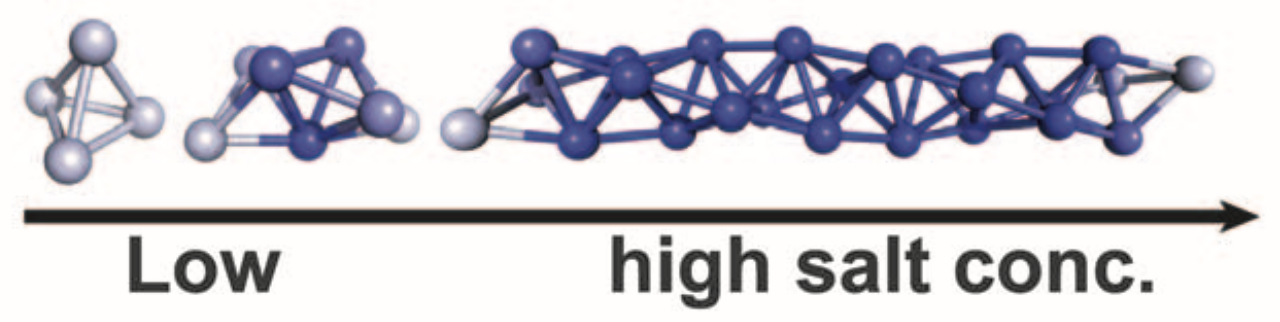
\includegraphics[width=0.44\textwidth]{Figures/fig2A_Chen2011_Science}}
%  \vspace{-5pt}
%\caption{\label{fig:helices_of_JPs}Formation of helices
%  of Janus particles as salt concentration increases from 3.8 mM NaCl
%  (left) to 5 mM NaCl (right)~\cite{Chen2011_Science}.}
%\end{wrapfigure}
%In experiments, Janus particles are often immersed in a solution of
%ions~\cite{Chen2011_Science} or surfactants~\cite{Goodwin2009}. In
%electrolytic solutions, the interaction between salt and Janus particle
%gives rise to a slip velocity (on the particle surface) that depends on
%the ion distribution and the zeta potential~\cite{BayatiNajafi2016_JCP}
%(the potential difference between the Janus particle surface and the
%surrounding conducting fluid). The short-range interactions between
%Janus particles depend on the salt concentration: At very low salt
%concentrations, Janus particles repel one another electrostatically,
%whereas at high salt concentration, van der Waals forces cause Janus
%particles to aggregate irreversibly~\cite{Goodwin2009}. At intermediate
%concentrations of monovalent salt (NaCl), Janus particles are found to
%assemble in the form of a small number of elemental units of building
%blocks~\cite{Chen2011_Science}. Figure~\ref{fig:helices_of_JPs} shows
%that Janus particles can assemble into a helix at high concentration of
%monovalent salt when the volume fraction of Janus particles is low to
%moderate. At high volume fraction, helices of Janus particles form
%wormlike structures whose lifetimes allow fusion of
%helices~\cite{Chen2011_Science}. 

The PIs investigated how 
distinct morphologies can be obtained from 
the HAP model by shifting the boundary condition $g$ \cite{fu-ryh-qua-you2022}.
Consider the linear case where $f(\eta) = \eta^2$.
This choice makes \eqref{eq:SL} a boundary value
problem for the screened-Laplace equation
and the solutions have a boundary layer structure that decays to $0$ in the
bulk with the decay length $\rho$.
We consider three kinds of boundary conditions
on particle $\Gamma_i$:
\begin{equation}
  \label{eq:bcs}
  \begin{tabular}{c|c|c}
     \text{(a)} & \text{(b)} & \text{(c)} \\
    \hline
    \rule{0pt}{4ex} 
      $g(\mathbf{x}) = \displaystyle \frac{1+\cos (\theta_i(\xx))}{\sqrt{3\pi r}}$
    & $g(\mathbf{x}) = \displaystyle \frac{2+\cos (\theta_i(\xx))}{\sqrt{9\pi r}}$
    & $g(\mathbf{x}) = \displaystyle \frac{\cos (\theta_i(\xx))}{\sqrt{\pi r}}$
\end{tabular}
\end{equation}
The number $\theta_i(\xx)$ is the angle formed by the position $\xx$, the
particle center $\aa_i$, and the particle director $\dd_i$ (Figure \ref{fig:flow_map}).
The normalizations e.g., $(\pi r)^{-1/2}$, provide a uniform
surface energy $\int_{\Gamma_i} g^2 \,ds = 1$ for circular particles
of radius $r$. 
The cases (b) and (c) are obtained by applying a vertical shift
and scaling to case (a).
%, see Figure \ref{fig:bcs}.
Using this setup, the PIs simulate the dynamics of 100 particles with random
initial position and orientation, see Figure~\ref{fig:self-assembly2}.

%%\begin{wrapfigure}[9]{r}{0.65\textwidth}
%%  \vspace{-20pt}
%%  \begin{center}
%%  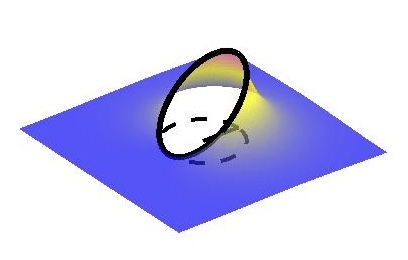
\includegraphics[width=0.2\textwidth]{figures/SpecificAim1/LPA.jpg}
%%  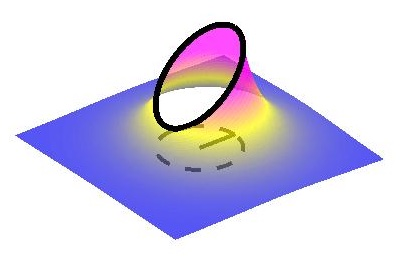
\includegraphics[width=0.2\textwidth]{figures/SpecificAim1/LPB.jpg}
%%  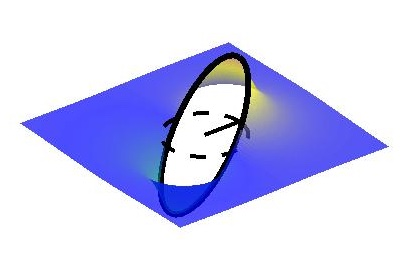
\includegraphics[width=0.2\textwidth]{figures/SpecificAim1/LPC.jpg}
%%  \end{center}
%%  \vspace{-20pt}  
%%  \caption{\label{fig:bcs} Boundary conditions characterize the water
%%    structure at the particle interface: an amphiphilic particle (left),
%%    a hydrophobic
%%  particle with anisotropic intensity (middle), a water structure with
%%  positive/negative charge (right). The dashed curve is the boundary of the
%%  disk and the arrow is its director for each particle.}
%%\end{wrapfigure}
%%
%\begin{wrapfigure}[15]{l}{2in}
%  \vspace{-4pt}
%  \centering
%  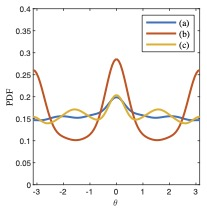
\includegraphics[width=2in]{figures/SpecificAim1/OrderPDFs.jpg} 
%  \vspace{-20pt}
%  \caption{\footnotesize
%    \label{fig:OrderPDFs}
%    Probability density functions for
%    relative orientation of nearby particles
%    for the data in 
%    Figure~\ref{fig:self-assembly2}, long time.
%  }
%\end{wrapfigure}
%%
Case (a) models amphiphilic particles.
Amphiphilic particles have a hydrophobic tail and a hydrophilic head: The hydrophilic side takes the value $\eta =0$.
This mimicks the apolar head of a lipid, for example, which does
not alter the structure of adjacent waters. The hydrophobic side
represents hydrocarbons and takes the value 
$\eta > 0$. The interaction between amphiphilic particles is attractive,
and they will collectively orient their tails toward
one another. 
PIs BQ, RR and YNY's previous work showed that this   
boundary condition produces two-dimensional micelles and
bilayers~\cite{Fu2018_SIAM}, as illustrated in 
Figure~\ref{fig:self-assembly2}(a).


Multilamelar bilayers arise when both sides of the particle
are hydrophobic (Figure~\ref{fig:self-assembly2}(b)).
The boundary condition \eqref{eq:bcs}(b) 
gives a particle with a hydrophobic intensity that is greater
on the $\theta_i = 0$ side than on the $\theta_i = \pi$ side.
The initial self-assembly is similar to that in case (a).
The difference arises in the long-time dynamics where the bilayers
no longer remain well-separated. 
Rather, the bilayers form layers 
as a consequence of the interfacial tension of exposed particle
heads~\cite{Huetal19, deMeetal21}. 

Finally, boundary condition \eqref{eq:bcs}(c) models 
a particle whose head surface repels the tail surface as proposed in
\cite{MaRa76, Ma77}.
The particles initially form chains with their directors perpendicular to the
length of the chain. The equilibrium structure
resembles a checkerboard pattern
where each particle coordinates
its head with the head of three other particles and its tail with the
tail of three other particles Figure~\ref{fig:self-assembly2}(c).
%
PIs' recent analyses in \cite{fu-ryh-qua-you2022} show that these patterns may be understood by a mixture of polar and nematic characteristics of the individual amphiphilic granuels, 
tuned by the boundary condition $g({\bf x})$, and lead to the following problem:
%
\begin{quotation}
  \noindent
  \textbf{Problem 6.} Can the collective dynamics of amphiphilic granuels with different boundary conditions 
be predicted by a coarse-grained model based on the kinetic theory?
\end{quotation}

%\begin{figure}[h!]
%  \begin{center}
%    \begin{tabular}{m{0.1cm}m{1.8in}m{1.8in}m{1.8in}}            
%      (a)
%    &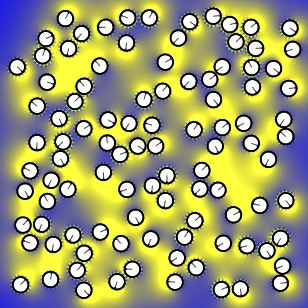
\includegraphics[width=1.8in]{figures/SpecificAim1/N100B1.jpg}
%    &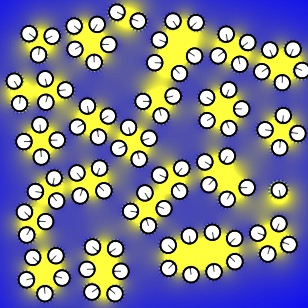
\includegraphics[width=1.8in]{figures/SpecificAim1/N100B2.jpg}
%     &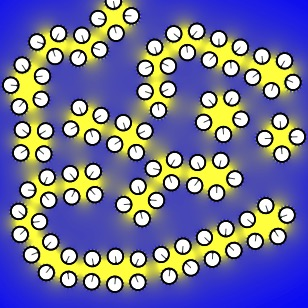
\includegraphics[width=1.8in]{figures/SpecificAim1/N100B3.jpg}    \\
%     (b)
%    &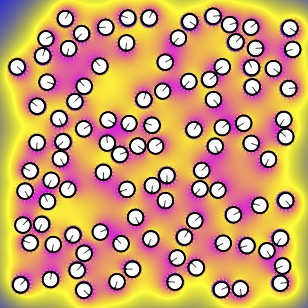
\includegraphics[width=1.8in]{figures/SpecificAim1/N100C1.jpg}
%    &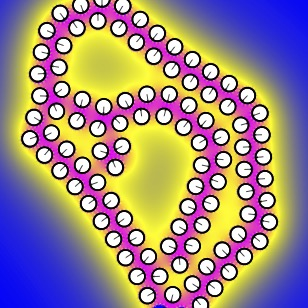
\includegraphics[width=1.8in]{figures/SpecificAim1/N100C2.jpg}
%      &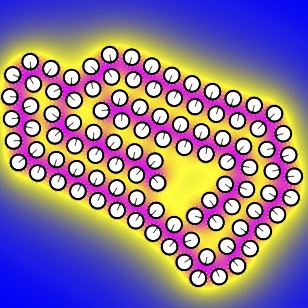
\includegraphics[width=1.8in]{figures/SpecificAim1/N100C3.jpg}    \\
%    (c)
%      &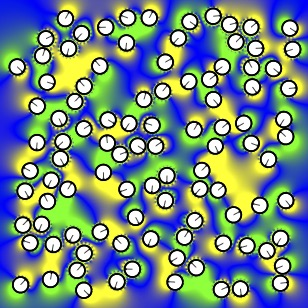
\includegraphics[width=1.8in]{figures/SpecificAim1/N100A1.jpg}
%      &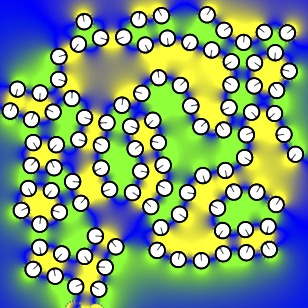
\includegraphics[width=1.8in]{figures/SpecificAim1/N100A2.jpg}
%      &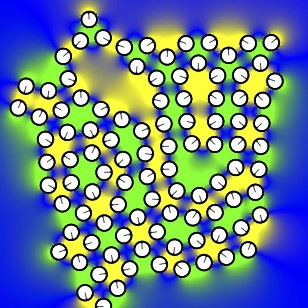
\includegraphics[width=1.8in]{figures/SpecificAim1/N100A3.jpg}    \\
%      &\multicolumn{1}{c}{$t = 0$}
%      &\multicolumn{1}{c}{intermediate time}
%      &\multicolumn{1}{c}{long time}
%  \end{tabular}
%  \end{center}
%  \vspace{-20pt}
%  \caption{\footnotesize
%    \label{fig:self-assembly}
%    Rows (a)-(c) have the same initial configuration
%    but have different boundary conditions $g.$ 
%    In row (a), self-assembly with an amphiphilic boundary
%    condition \eqref{eq:bcs}(a) results in a bilayer pattern shielding
%    the hydrophobic core (yellow, $u > 0$) from the aqueous phase (blue, $u = 0$).
%    Row (b) shows particles with a hydrophobic intensity that is
%    greater on one side of the particle (magenta) than the other (yellow).
%    In row (c), green is for $u < 0$, yellow is for $u > 0$, and blue is for $u = 0$.
%    Particles orient like sides to form a checkerboard pattern.\\
%  }
%\end{figure}

PI Young proposes to construct a kinetic theory to quantify the underlying mechanisms that lead to distinct morphologies of granuels described above.
Consider the suspension dynamics on a length scale much longer than the particle size, and denote the number density of 
amphiphilic granuels at time $t$ with position ${\bf x}$ and director vector ${\bf p}$ ($|\bf p|=1$) as $\psi({\bf x}, {\bf p},t)$, which satisfies the 
Smoluchowski equation 
\begin{align}
\frac{\partial \psi}{\partial t} &= -\nabla_{\bf x} \cdot\left(\psi\dot{\bf x}\right) - \nabla_{\bf p}\cdot\left(\dot{\bf p}\psi\right),\\
\dot{\bf x} &= {\bf u} + {\bf F}\left(\eta,{\bf p}\right) - D_x\nabla_{\bf x}\ln\psi,\\
\label{eq:dpdt}
\dot{\bf p} &= \left({\bf I}-{\bf p}{\bf p}\right)\cdot\nabla {\bf u}\cdot {\bf p} + {\bf G}\left(\eta,{\bf p}\right) - D_p \nabla_{\bf p}\ln \psi + \frac{{\bf H}}{\gamma},\\
{\bf H} &\equiv -\frac{\delta {\cal F}}{\delta {\bf p}} = -\frac{\delta}{\delta {\bf p}} 
\int d{\bf x} \left\{\frac{K_p}{2} \left(\vec\nabla{\bf p}\right)^2 + \frac{K}{2}\left(\nabla\left({\bf p}{\bf p}^T- \frac{\bf I}{2}\right)\right)^2\right\},
\end{align}
where the subscripts denote the variables the derivative is taken with respect to, 
$D_x$ is the translational diffusion and $D_p$ is the rotational diffusion. 
 ${\bf F}\left(\eta,{\bf p}\right)$ and ${\bf G}\left(\eta,{\bf p}\right)$ are the drift and rotation induced by the potential $\eta$ and alignment, respectively.
 They can be derived using the reciprocal theorem as in the case of 
the phoretic Janus particle suspension \cite{TraversoMichellin2020_PRF,TraversoMichellin2022_JFM}.
The last term in equation~(\ref{eq:dpdt}) characterizes the relaxation of the director alignment to the minimum of the
free energy ${\cal F}$, where the parameter $K_p$ controls the alignment of directions, and $K$ characterizes the alignment of orientations:
$K=0$ and $K_p > 0$ when the suspension is purely polar, and $K_p=0$  and $K>0$ when the suspension is purely nematic \cite{Amiri2022_JPhysA}. 
%
Case (a) (boundary condition (\ref{eq:bcs})(a)) corresponds to a balanced mixture of polar and nematic characteristics of the nematic particles.
Case (b) corresponds to a polar suspension, while case (c) corresponds to a nematic suspension. 

PI Young has used the kinetic theory to investigate the many behaviors of droplets of
nematic fluids \cite{YoungShelleyStein2021_MBE}. 
The kinetic-theory based coarse-grained model for active suspension has been shown to work reasonably well beyond the dilute limit \cite{Saintillan2018_ARFM}.
Within this framework, the stress on the viscous solvent from the amphiphilic granuels can be computed
by integrating the stress from the single particle weighted by the density distribution $\psi$ over the whole domain \cite{TraversoMichellin2020_PRF,TraversoMichellin2022_JFM}.
In particular, PI Young proposes to use the Bingham closure \cite{YoungShelleyStein2021_MBE} to approximate these calculations to study the
dynamics and rheology of suspension of amphiphilic granuel controlled by tuning the boundary conditions on the microscopic amphiphilic granuels, 
which the PIs recently investigated using direct numerical simulations and the results are summarized in \cite{fu-ryh-qua-you2022}. Working together with PIs Quaife and Ryham, the team proposes to extract the coefficients
$K$ and $K_P$ for a single granuels first from the direct numerical simulation results. Using these values, the dynamics, pattern formation and rheology
predicted from analyzing the proposed coarse-grained model will be compared quantitatively against numerical simulations. 

It is possible that the outcome of the proposed quantitative comparison depends on the treatment of collisions between amphiphilic granuels 
in the simulations (see \S~\ref{sec:specificaim2}), 
and the modeling of the steric interactions in the kinetic theory. If this turns out to be an important effect, PI Young will incorporate the formulation of constraint forces as part of the active stress in the Stokes equations for the suspension.  Such constraint forces arise from the geometric 
constraint that the amphiphilic granuels cannot overlap with each other \cite{Weady2022_PRF}. 

 
%The ultimate goal is to use numerical simulations to aid
%the syntheses of soft matter materials.
%Here, mathematical models like the kind we propose are crucial
%because the model parameters control surface properties independently, 
%which can be difficult to accomplish experimentaly 
%~\cite{Bradley2016,Mallory2017,Bradley2017}.
%The ability to translate phenomenological parameters
%into measurable quantities is important. 
%For example, Figure~\ref{fig:OrderPDFs} plots
%the probability density function for 
%relative orientation of adjacent particles
%for the three boundary condition cases:
%(a) is unimodal with a peak at $\theta = 0$,
%(b) is bimodal with peaks at $\theta = 0$ and $\theta = \pi$,
%and (c) is multimodal with peaks at $\theta = 0$ and $\theta = \pm \pi/2$.
%This kind of information can be used as an indicator
%of the collective morphology. As another example,
%it is costly or difficult to manufacture
%Janus particles with uniform shape.
%Thus, we can replace the idealistic boundary
%conditions \eqref{eq:bcs} with a more realistic one like
%\begin{equation}
%\label{eq:vonMises}
%  g_i(\xx) = \sqrt{
%  \frac{\exp( \kappa_i\cos(\theta_i(\xx) - \theta^0_i))}
%  {2\pi r_i I_0(\kappa_i)}}.
%\end{equation}
%Here, the term under the square root is the von Mises distribution with
%director angle $\theta^0_i$ and Bessel function $I_0$ of order zero~\cite{Fisher_1993}.
%The square of this function is asymptotic to a normal distribution with variance
%like $1/\kappa_i$, $\kappa_i \to \infty$. We can replicated surface imperfections
%by randomizing the concentration $\kappa_i$ and particle radii $r_i$,
%for example.

%\subsubsection{Dynamics of a pair of Janus particles in ionic
%solutions\label{subsubsec:JP_electrolyte}}
%We propose to investigate the effects of ion transport and distribution
%on the self-assembly of Janus particles within the HAP framework as
%follows. First the Stokes equations are modified to incorporate the
%transport of ions as
%\begin{equation}
%\label{eq:EKstokes}
%\begin{aligned}
%  &-\Delta \mathbf{u} + \nabla p = \Delta\psi\cdot\nabla\psi, \qquad
%  \nabla \cdot \mathbf{u} = 0,  \quad \mathbf{x} \in \Omega,\\
%  &\delta^2\Delta\psi = -\frac{1}{2}\left(n_+-n_-\right),\qquad
%  \frac{\partial n_{\pm}}{\partial t} + \nabla\cdot{\bf j}_{\pm} = 0,\qquad {\bf j}_{\pm} = -\nabla n_{\pm} \mp n_{\pm} \nabla\psi + \mbox{Pe} n_{\pm}\mathbf{u},
%\end{aligned}
%\end{equation}
%where $\psi$ is the electric potential, $\delta$ is the ratio of Debye
%screening length (inversely proportional to the square root of ion
%concentration) to the particle size, $\mbox{Pe}$ is the Peclet number, a
%ratio between the convection and thermal diffusion time scales, and
%$n_{+}$ and $n_{-}$ are the concentration of cation and anion respectively.
%In the limit
%of small $\delta$, PI YNY and collaborator Y.~Mori (U Penn) used
%asymptotic analyses to show that the jump in electric potential across
%the interface (zeta potential on the Janus particle surface) may give
%rise to different physical consequences such as
%electrophoresis~\cite{Mori2018_JFM}.
%%
%An important question to address is: {\it How would such electrophoresis
%be affected by the HAP between two Janus particles?} As the first part
%of Specific Aim 3, we will address this important question. Results from
%this effort will help elucidate the effects of salt concentration on the
%assembly of Janus particles (\S\ref{subsubsec:em_effects}).
%
%We will couple the electrokinetics in~\eqref{eq:EKstokes} with the
%mobility problem of Janus particles in a viscous solvent through the
%velocity field, ion distribution, and the hydrophobic potential. First
%the screen length $\rho$ and the potential $f(u)$ in the HAP model are now 
%dependent on  the ion concentrations. 
%%
%Second the value of the HAP may depend on the distribution of ions and
%electric potential right next to the particle
%surface~\cite{Mori2018_JFM}. Within this framework, we will first
%investigate the interaction between two Janus particles under HAP in an
%electrolytic solution described by the above equations. We will conduct
%analytical calculations to investigate the effects of ion transport on
%the hydrophobic attraction between two Janus particles using the
%reciprocal theorem as in~\cite{BayatiNajafi2016_JCP} for two Janus
%particles with a small surface activity.
%
%
%\subsubsection{Electromechanical effects on the dynamic assembly of Janus particles \label{subsubsec:em_effects}}
%Results from the proposed work in \S\ref{subsubsec:JP_electrolyte} will
%shed light on how the electrokinetics described in~\eqref{eq:EKstokes}
%may be simplified to a dielectric-like model where the bulk charges are
%constant, and the fluid flow and particle mobility are determined by the
%surface charge and the zeta potential as shown in~\cite{Mori2018_JFM}.
%Under such simplification, equation~\eqref{eq:EKstokes} may be
%re-formulated into integral forms. PIs RR and YNY will conduct the
%asymptotic analyses to derive this form, and work with PI BQ to design
%numerical algorithms to simulate the modified system. We will first
%investigate the effects of salt concentration on the assembly of Janus
%particles to form helices, as shown in Figure~\ref{fig:helices_of_JPs}.
%
%With these results, the PIs will be ready to make quantitative
%connections between a Janus particle membrane and a lipid bilayer
%membrane in an electrolytic solution. In recent
%experiments~\cite{FaizEtAl2019_SoftMatt}, membrane bending rigidity was
%determined as a function of lipid composition from 0 to 100 mol $\%$ of
%charged lipids using flicker spectroscopy of the shape fluctuations of a
%giant unilamellar vesicle (GUV). Membrane bending rigidity increases
%with increasing lipid surface charge, but decreases with increasing salt
%concentration in the bulk solution due to the screening of the lipid
%surface charge. This result agrees with several theoretical
%models~\cite{Kralchevsky1996_JCIS, May1996_JChemPhys,
%LoubetEtAl2013_PRE} that also assume the quadratic form of the elastic
%energy density in the presence of surface charge and bulk
%charge~\cite{DuplantierGoldstein1990_PRL, Winterhalter1992_JPC}.
%%As the
%%electrostatic interaction is non-local in nature, we expect that the
%%controversy of the HK elastic energy form (see
%%\S\ref{subsec:specific_aim_1}) would worsen in the presence of
%%electrostatic interactions and electrokinetics.
%The PIs will extend the
%approaches in \cite{Fu2018_SIAM} to charged lipids to
%calculate the bending moduli and compare against the experimental
%results in~\cite{FaizEtAl2019_SoftMatt}. We propose to incorporate an
%explicit surface charge on each particle boundary $\Gamma_i$ and compute the
%electrostatic potential as a functional of particle configuration.  By
%adding the electrostatic force to the hydrophobic attraction force
%between particles, we will assess the dependence of elastic moduli on
%electric charges using the methods described in \cite{Fu2018_SIAM}. Results from these proposed calculations
%will provide further comparisons and validations of the HAP model
%against the continuum mechanics.
%
%Once the effects of lipid charges on the moduli are verified, the PIs
%propose to examine how to use an external electric field to control the
%amphiphilic self-assembly in solvent. PI YNY has a track record of
%working on electrohydrodynamics of an elastic, inextensible membrane
%using both asymptotic analysis~\cite{Nganguia2013_PRE, Young2014_JFM,
%Young2015_PoF} and numerical simulations~\cite{Nganguia2015_CiCP} and
%will work with both PIs RR and BQ to extend the HAP model to study the
%electromechanical effects on the assembly of colloidal amphiphiles.
%Results from this research will yield a quantitative understanding of
%how to utilize an electric field to achieve optimal control of assembly
%of amphiphiles in solvent.




